\chapter{Verfahren zur Metallbearbeitung und Grundlagen der Elektrotechnik}
\label{cha:Metallbearbeitung und Elektrotechnik}

\section{Erstellung verschiedener Werkstücke aus Metall}

Es sind die wichtigsten Grundlagen zur Metallbearbeitung zu erlernen. Dazu sollen zunächst händische Verfahren erlernt werden, um anschließend Methoden 
zur maschinellen Bearbeitung kennen zu lernen. Schwerpunkt in dieser Aufgabe besteht darin, Fertigungsverfahren aus dem Bereich Zerspannung, Umformung 
und Fügung an Problemstellungen anzuwenden. Des Weiteren sollen Kenntnisse über die wichtigsten Eigenschaften verschiedener Metallarten erlernt werden. 
Außerdem ist es wichtig, dass Vorschriften zum Arbeitsschutz eingehalten und stets mit Bedacht behandelt werden. 
\\
Ziel ist eine angeleitete, aber selbstständig durchgeführte Lösung eines Problems, mithilfe der einzelnen Bearbeitungsverfahren durchführen zu können. 
\clearpage

\section{Werkstückherstellung mithilfe verschiedener Metallbearbeitungsverfahren}

In der Metallverarbeitung gibt es verschiedene Verfahren zur Herstellung eines Werkstückes. Diese Verfahren werden in Hauptgruppen zusammengefasst und
unterscheiden sich in ihren Eigenschaften der Bearbeitung und Veränderung von Rohmaterialien.
\\
Eines dieser Verfahren ist das Trennen. Hierbei handelt es sich um ein spanendes Fertigungsverfahren.
\\
Die spanende Fertigung beschreibt ein Verfahren zur Bearbeitung verschiedener Werkstoffe mit Hilfe von Werkzeugen, bei denen Material vom Werkstoff 
herausgeschnitten wird, um dessen Form oder Oberfläche zu verändern. Das abgetragene Material wird auch als Span bezeichnet.
Zu den spanenden Fertigungsverfahren zählen \zB das Feilen, Schleifen, Sägen, Bohren, Drehen und Fräsen. Jedes dieser Verfahren hat seine eigenen 
Eigenschaften und bietet sowohl Vor- als auch Nachteile.\autocite{Dietrich.2020}
\\\\
Das Feilen wird meist von Hand ausgeführt, mit sogenannten Werkstattfeilen und dient zur präzisen Bearbeitung von Werkstücken. Eine Werkstattfeile hat
wie im Bild zu sehen einen Griff, an dem das Blatt befestigt ist. Auf diesem Blatt gibt es Einkerbungen, welche auch wie Zähne aussehen können. Diese 
sogenannten Hiebe, welche maschinell in das Blatt gefräst werden oder von Hand eingeschlagen werden, sorgen für den Abtrag des Materials an dem zu 
bearbeitenden Werkstück. Dies hat zur Folge, dass nur kleinere Arbeiten mit der Feile getätigt werden können, da andernfalls dieses Verfahren zu 
zeitaufwendig ist. Im Gegensatz zur maschinellen Bearbeitung, wie \zB beim Fräsen oder Drehen, bietet dass Feilen den großen Vorteil, dass auch filigrane 
Arbeiten auf engem Raum getätigt werden können.
\begin{figure}[hbt]
    \centering
    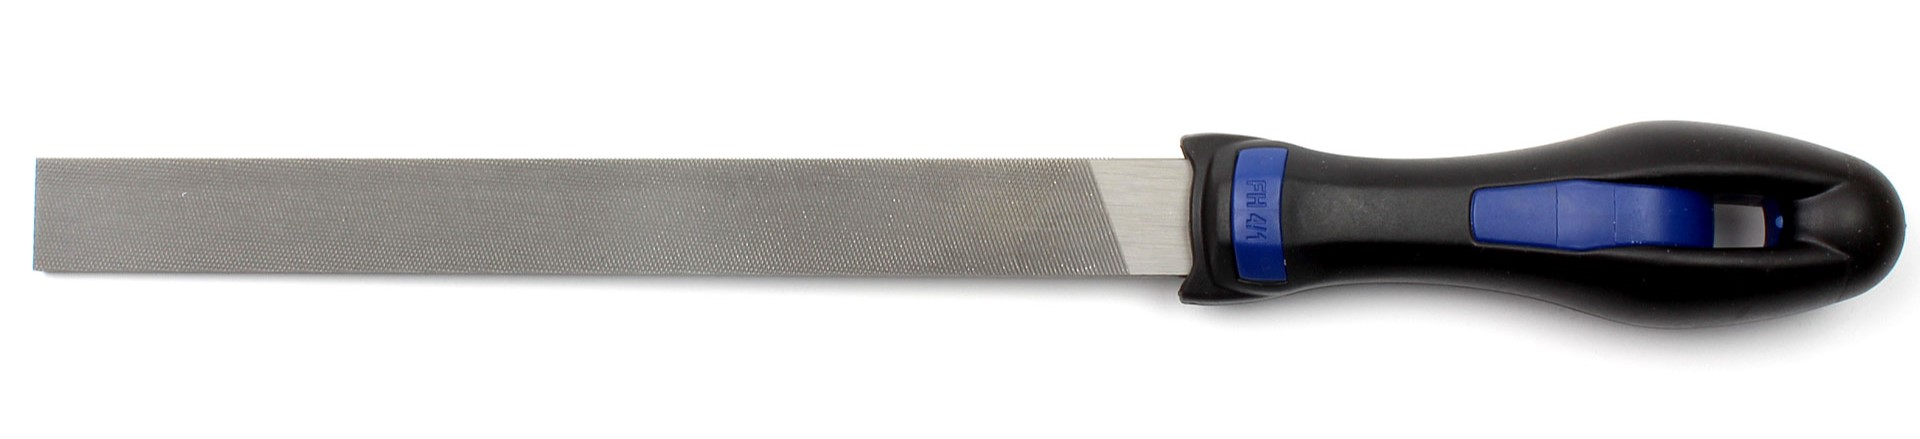
\includegraphics[width=1\linewidth]{images/Werkstattfeile}
    \caption[Werkstattfeile]{Werkstattfeile \autocite{Werkstattfeile}}
    \label{fig:Werkstattfeile}
\end{figure}
\\\\
Zudem unterscheiden sich Feilen in ihrer Hiebzahl. Diese gibt an, wie viele Zähne sich auf einem 
Centimeter des Blattes befinden. Es gibt Feilen mit wenigen Hieben, welche ihren Anwendungsbereich in der Bearbeitung von weichen Werkstoffen wie 
Aluminium haben, aber auch zur Grobbearbeitung genutzt werden, um möglichst viel Material abzutragen. Feilen mit einer großen Anzahl von Hieben tragen
nur wenig Material ab und sind meist ungeeignet für weiche Werkstoffe, da die Späne in den Zwischenräumen stecken bleiben, dafür erzeugen diese meist eine 
glatte Oberfläche mit einer höheren Güte. Die Güte ist eine Oberflächenangabe, welche zur Aussage bringt, wie rau oder glatt diese ist. \autocite{Forster.2018}
\\\\
Das Fräsen ist neben dem Drehen eines der wichtigsten Metallbearbeitungsverfahren. Die Verfahren unterscheiden sich in den Anwendungsbereichen und 
Bearbeitungsverfahren. 
\\
Hierbei sind Werkstücke, die gedreht werden immer symmetrisch, da ausschließlich Runde Werkstoffe verarbeitet werden können. Dies liegt daran, dass beim 
Drehen das Werkstück um die eigene Achse und beim Fräsen das Werkzeug gedreht wird. 
\\
Das Drehen wird \zB bei Bolzen, Schrauben oder Unterlagscheiben angewandt und das Fräsen bei \zB Nuten, Formänderungen oder Bohrungen. Heutzutage unterscheidet
man zwischen zwei Arten des Fräsens und Drehens, dem konventionellen und dem Computerized Numerical Control (CNC) Fräsen oder Drehen. Beide Verfahren bieten
einen sehr hohen Grad an Genauigkeit und finden einen großen Anwendungsbereich in der Fertigung präziser Werkstücke. Das Fräsen oder Drehen bringt den 
großen Vorteil mit sich, dass viel Material abgetragen werden kann, jedoch die Qualität des Werkstücks erhalten bleibt. Durch die CNC Technologie ist das 
Fertigen gleichaussehender Teile automatisiert und für den Fließbandbetrieb ideal. Dies bedeutet, dass es für die Fertigung höher Stückzahlen optimiert 
wurde. Somit bietet dies Unternehmen die Chance Kosten durch schnelle und präzise Fertigung zu reduzieren. Allerdings gibt es auch Nachteile beim Fräsen 
oder Drehen, da die Werkstoffe und Werkzeuge sehr großer Hitze ausgesetzt sind und somit die Gefahr
herrscht, dass sich die Eigenschaften \zB des Metalls negativ verändern. Jede Metallart hat ihre eigene Anordnung der
Atome, welche die Gitterstruktur ausbilden und durch Hitze verändert werden kann. Durch eine solche Änderung in der Anordnung können sich die 
Eigenschaften des Metalls verändern, \zB im Bereich der Umformbarkeit oder Bruchfestigkeit. Um diese thermische Belastung einzuschränken, werden oftmals 
Kühlflüssigkeiten verwendet. Diese bestehen aus einem Gemisch aus Öl und chemischen Zusätzen, welche die Eigenschaft mit sich bringen, gut Wärme 
aufzunehmen und ein gutes Schmierverhalten aufzuweisen. Dadurch wird die Reibung zwischen Material und Werkzeug minimiert, wodurch weniger Reibungswärme
entsteht. \autocite{Dietrich.2020} 
\\\\
Ein weiteres Verfahren zur Bearbeitung von Werkstoffen, ist die Umformung. Der große Unterschied zu spanenden Fertigungsverfahren ist hierbei, dass kein 
Material abgetragen wird, sondern die Form des Werkstücks verändert wird. Da die meisten Metalle die Eigenschaft einer guten Verformbarkeit haben, wird 
dieses Verfahren überwiegend in der Metallindustrie verwendet. Zu solchen Verfahren zählen \zB Walzen, Schmieden und Biegen. Das Verfahren ist einfach in der Anwendung und 
flexibel einsetzbar. Allerdings beschränkt sich dies auf einfache Problemstellungen, denn sobald ein komplexes Werkstück benötigt wird, reicht 
dieses Verfahren nicht mehr aus. Ein großer Nachteil beim Biegen ist, dass man einen Mindestbiegeradius einhalten sollte, da sich das Material sonst verjüngt 
oder gar bricht. Dies bedeutet, dass sich die Dicke des Materials an der biegenden Stelle stark verringert. 
Um dieses Verhalten zu unterbinden, sollte der Biegeradius vor Beginn der Arbeit beachtet werden. Dazu muss je nach Metallart ein Radius von ein- oder zweifacher
Stärke des Materials genommen werden. \autocite{Arendes.2023}
\\\\
Das letzte wichtige Verfahren ist das Fügen. Hierbei werden mindestens zwei Werkstücke zu einer dauerhaften Verbindung gefügt. Zu den wichtigsten 
Fügeverfahren zählt das Schweißen, welches in Unternehmen einen großen Anwendungsbereich findet. Sei es in der Verbindung und dem Bau von Rohren oder 
Schiffen, als auch in der Lösung von schnellen Problemen vor Ort, wie \zB zur Reparatur von Beschädigungen an Wasser- oder Gasrohren. Jeder Einsatzbereich 
hat andere Anforderungen an das Schweißen, was eine Vielfalt an Schweißmethoden und Verfahren voraussetzt. 
\begin{figure}[hbt]
    \centering
    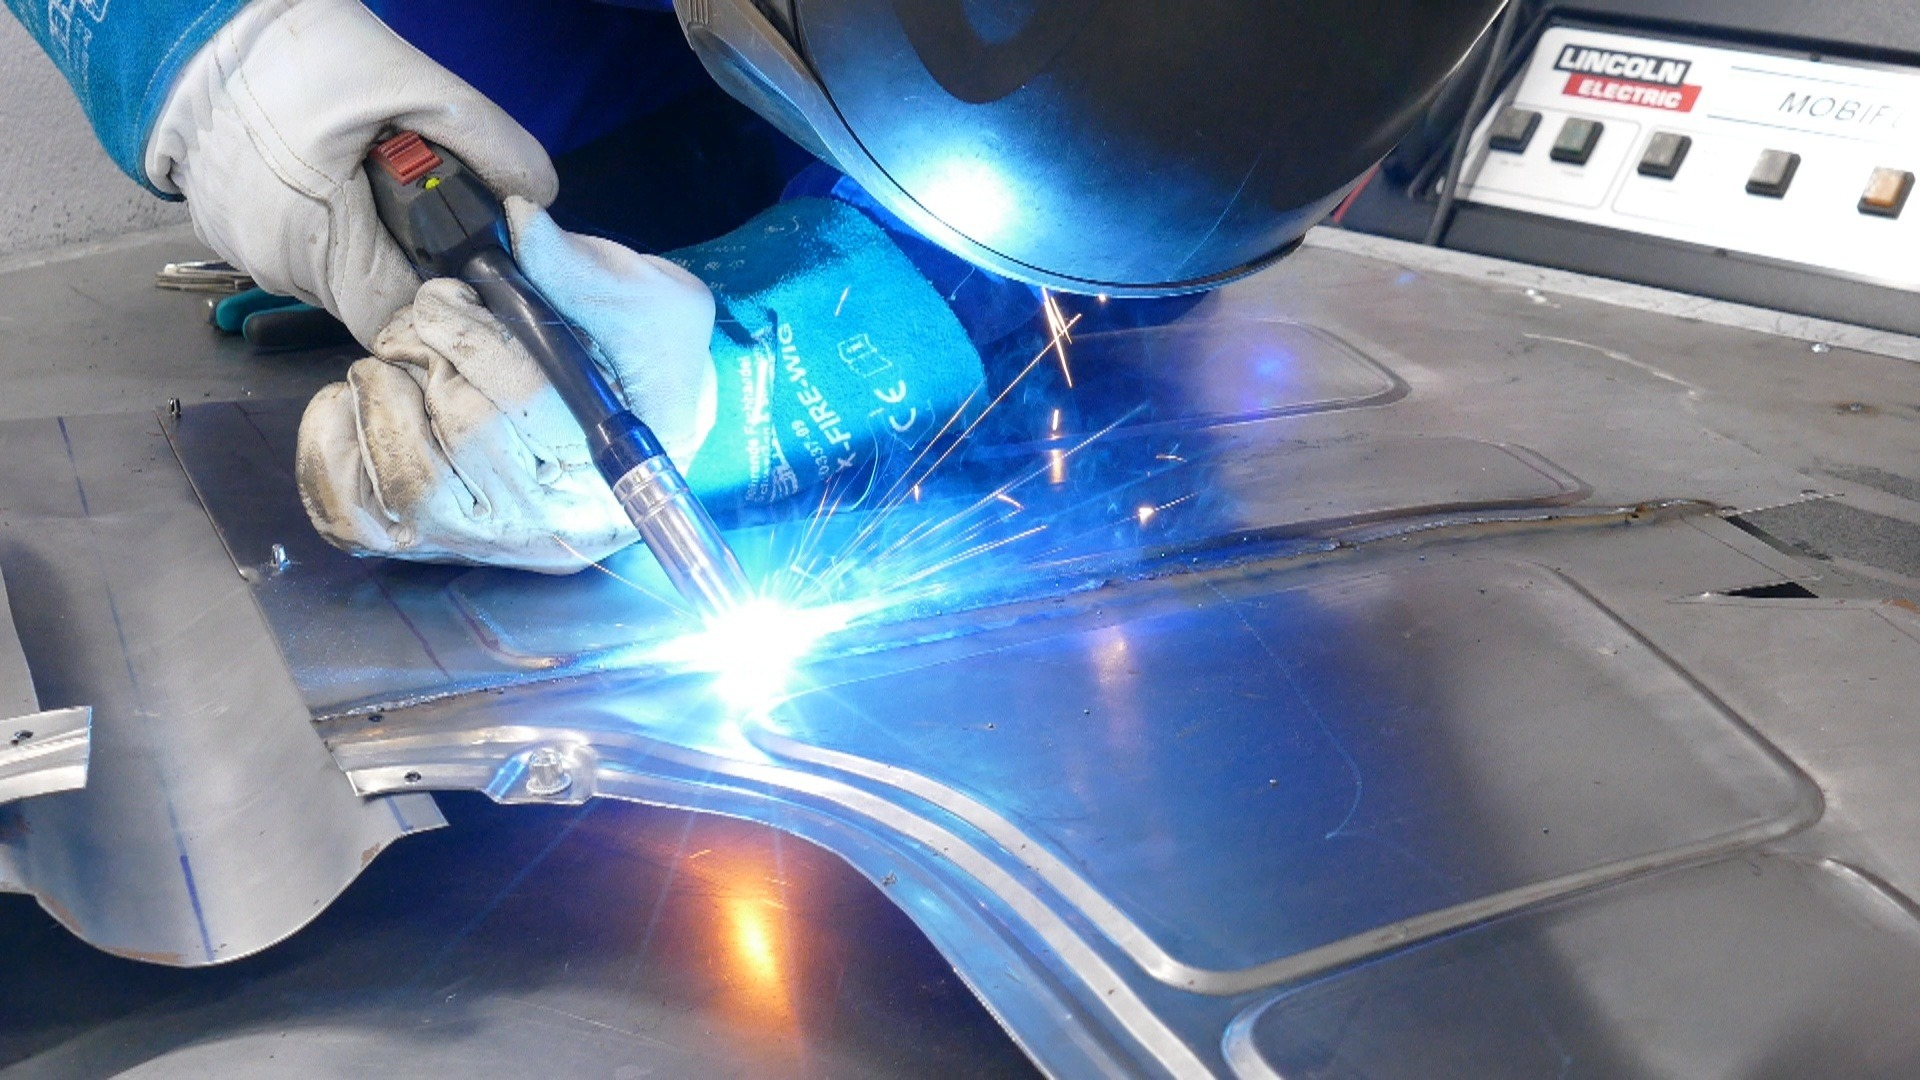
\includegraphics[width=0.98\linewidth]{images/MAG}
    \caption[MAG-Schweißen]{MAG-Schweißen \autocite{MAG}}
    \label{fig:MAG-Schweißen}
\end{figure}
\\Eines dieser Verfahren ist das 
Lichtbogenhandschweißen, in dem mit Hilfe elektrischen Stroms ein Lichtbogen erzeugt wird, der die Materialien schmilzt und bei anschließender Aushärtung 
miteinander verbindet. Ein Lichtbogen ist eine leitende Verbindung zwischen Metall und Schweißdraht über die Luft, bei der sehr hohe Temperaturen entstehen, 
welche zum Schmelzen des Drahtes und Metalls führen. Dieses sogenannte Schmelzbad muss durch Zufuhr von einem geeigneten Schutzgas, meist Argon umhüllt sein,
um eine Oxidation mit dem Umgebungssauerstoff zu verhindern. Bei einer Oxidation entsteht eine chemische Reaktion des Metalls mit dem Umgebungssauerstoff, 
bei der sich eine Verbindung zwischen Metall und Sauerstoff ausbildet. 
Chemische Reaktionen mit Sauerstoff werden im allgemeinen als Oxidationen bezeichnet.
Diese Oxidation würde zu einer Verschlechterung der Qualität und zu einer Versprödung der Schweißnaht führen. Dies hat zur Folge, dass diese nicht 
belastungsfähig ist.
Die Verwendung von Schutzgas wird nur in den Methoden des Metall-Inertgas- (MIG), Metall-Aktivgas- (MAG) und Wolfram-Inertgas-Schweißens (WIG) 
verwendet, da es bei diesen Methoden keine andere Möglichkeit zum Schutz des Schmelzbades gibt. Dieses sorgt bei MIG dafür, dass das Schmelzbad nicht mit dem 
Schutzgas reagiert. Dieses Inerte Verhalten beschreibt eine
Reaktionsträgheit, ganz im Gegenteil zum MAG-Schweißen. Hier ist es ein reaktionsfreudiges Gas, auch als Aktivgas bezeichnet, welches mit dem permanent 
nachgeführten Schweißdraht reagiert. 
Beim WIG-Schweißen wird ein Inertes Gas verwendet, um die Schweißspitze, welche aus Wolfram besteht vor Reaktionen zu
schützen, da diese nicht schmilzt. Bei dieser Methode erzeugt diese nur den Lichtbogen zwischen Metall und Spitze, wodurch das Metall schmilzt und gefügt 
werden kann, mithilfe von externer Drahtzugabe. Diese drei Methoden bieten den großen Vorteil einer hohen Produktivität, wie auch eine gute Automatisierung,
da der Schweißdraht von einer Trommel automatisch und kontinuierlich zugeführt wird. 
\clearpage

Im Gegensatz zu diesen Methoden steht das Elektrohandschweißen mit
einer Stabelektrode. Hierbei wird kein Schutzgas benötigt, da sich das Schweißbad durch die entstehende Schlacke und den Rauch selbst vom 
Umgebungssauerstoff isoliert. Die Stabelektrode ist ein Metallstab, welcher von einem Brennstoff umhüllt ist, der die Reaktion beim Schweißen fördert und 
für die Isolierung des Sauerstoffes sorgt.
\begin{figure}[h]
    \centering
    \includegraphics[width=0.98\linewidth]{images/Elektrodenschweißen}
    \caption[Elektrodenschweißen]{Elektrodenschweißen \autocite{E-Hand}}
    \label{fig:Elektrodenschweißen}
\end{figure}
\\Beim Schmelzen dieses Stabs entsteht das Nebenprodukt Schlacke, welches sich auf dem geschweißten Metall 
absetzt und dieses isoliert, bis es vollständig ausgehärtet ist.  Dies bietet dem Anwender den großen Vorteil, dass diese Methode nahezu überall anwendbar
ist und keine großen Geräte mit Schutzgaszufuhr benötigen. Deshalb wird diese Methode auch häufig im Außenbereich angewandt. Der größte Nachteil ist 
hierbei die hohe Rauchentwicklung und das Entfernen der Schlacke. Hierzu sollte in geschlossenen Räumen immer eine Absaugung gewährleistet sein, da die
Dämpfe gesundheitsschädlich sind.  Zudem ist es beim Schweißen allgemein von hoher Relevanz, dass ein Augenschutz, wie auch eine geeignete persönliche 
Schutzausrüstung (PSA) getragen wird, um sich vor Funken und Strahlung durch den Lichtbogen zu schützen. \autocite{Spath.2023}
\clearpage


\section{Erstellung von elektrischen Schaltungen}

Im Bereich der Elektrotechnik sollen grundlegende Kenntnisse erlernt werden. Dazu sollen Problemstellungen zunächst theoretisch 
betrachtet werden, um diese dann Anhand von Versuchsaufbauen praktisch zu betrachten. Dies findet zunächst im Bereich der Gleichstromlehre statt und 
wird anschließend m Drehstrombereich behandelt. Hier ist es von entscheidender Rolle, dass auch wichtige Regeln und Vorschriften zur Arbeitssicherheit 
erlernt und beachtet werden, um Arbeitsunfälle zu verhindern.
\\
Ziel ist eine eigenständige Bearbeitung von Problemstellungen und das Erlernen von neuen elektrotechnischen Grundlagen, welche als Hilfestellung zur 
zielorientierten Bearbeitung dienen. 
\clearpage

\section{Die Integration von Elektrotechnik in den beruflichen Alltag}

Im Folgenden geht es um die Lösung von Problemen im Bereich der Elektrotechnik. Hierzu bezieht sich der erste Teil auf die Lösung von Gleichstromproblemen und der 
zweite Teil auf die Lösung von Wechsel- bzw. Dreiphasenwechselstromproblemen. In der Gleichstromlehre gibt es \zB Formeln für Parallel oder in Reihe 
geschaltete Widerstände, die Kirchhoffschen Gesetze oder das ohmsche 
Gesetz. Diese Formeln dienen dazu, dass Verhalten von Widerständen zu beschreiben, um daraus praktische Schlüsse in der Anwendung dieser zu ziehen. 
Die Kirchhoffschen Gesetze befassen sich mit dem Verhalten von Spannung, Strom und Widerstand bei geschlossenen Stromkreisen oder einzelnen Punkten, an denen 
mehrere Kabel zusammenlaufen, den sogenannten Knotenpunkten. Das ohmsche Gesetz dient zum Berechnen des Verhaltens an statischen Punkten im Stromkreis und 
beschreibt das Verhalten zwischen Strom, Spannung und Widerstand. Ein Widerstand hat unter anderem den Nutzen, die Spannung oder den Strom zu verringern, um 
den Verbraucher zu schützen. Je nachdem, welches Problem zu lösen ist, muss der Widerstand parallel, in Reihe oder beides in Kombination verwendet werden. 
Da es allerdings nur festgelegte Widerstandgrößen zu kaufen gibt und meist auch nicht alle im Unternehmen vorhanden sind, müssen verschiedene Größen miteinander
kombiniert werden. Durch die Verwendung der Formel für parallelgeschaltete Widerstände, kann man \zB durch die Verwendung zweier 100 $\Omega$ Widerstände 
herausfinden, dass dadurch ein 50 $\Omega$ Widerstand entsteht. 
%\clearpage
Dies kann beliebig oft angewandt werden, wobei die Formel 1.1 zur Berechnung von parallelen Widerständen nur für eine maximale Anzahl von zwei 
Widerständen und die Formel 1.2 für eine unbegrenzte Anzahl von Widerständen zählt.
\begin{equation}
R_{\text{ges}}=\frac{R_1 \cdot R_2}{R_1+R_2}
\label{eqn:Parallelschaltung von 2 Widerständen}
\end{equation}
\begin{equation}
\frac{1}{R_{\text{ges}}}=\frac{1}{R_1}+\frac{1}{R_2}+\dots
\label{eqn:Parallelschaltung von mehreren Widerständen}
\end{equation}
Zudem ist bei parallelgeschalteten Widerständen zu beachten, dass die Spannung, welche über den Widerständen abfällt gleich bleibt und diese Art der 
Verschaltung zu einer Reduktion des Stroms führt. Um den gesamten Strom über den Widerständen zu berechnen, kann folgende Formel angewandt werden.
\begin{equation}
I_{\text{ges}} = \frac{U}{R_{\text{ges}}}
\label{eqn:Gesamtstrom Parallelschaltung}
\end{equation}
Bei einer Reihenschaltung von Widerständen ist die Berechnung deutlich einfacher, da sich diese lediglich addieren. Somit können beliebig viele Widerstände in 
Reihe geschaltet werden, um den Gesamtwiderstand zu erhöhen.
\begin{equation}
R_{\text{ges}}=R_1+R_2+\dots
\label{eqn:Widerstand Reihenschaltung}
\end{equation}
Allerdings ist bei einer Reihenschaltung zu beachten, dass eine Reduktion der Spannung über den Widerständen stattfindet, weshalb dieser Typ Verschaltung 
angewandt wird bei Verbrauchern, die eine geringere Spannung benötigen, als die anliegende. Zudem ist es möglich beide Typen der Verschaltung zu kombinieren. 
Hierbei ist dann jeweils zu beachten, welche der Formeln angewandt werden muss, da beide Typen vorhanden sind. Wichtig dabei zu beachten ist, dass das 
Schaltbild in einzelnen Teilschritten berechnet wird und die beiden Formeln für die Reihen- und Parallelschaltung nicht vermischt werden.
Allgemein gilt, dass von innen nach außen gerechnet wird. Im folgenden Beispiel wird eine solche Schaltung nochmals genauer erläutert.
\begin{figure}[hbt]
    \centering
    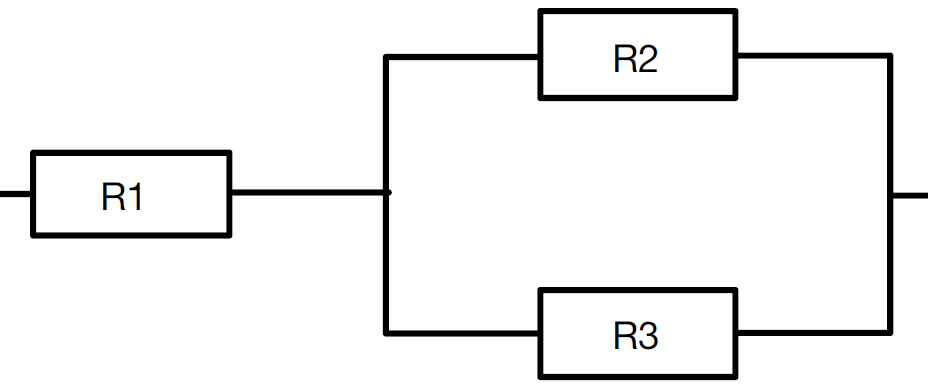
\includegraphics[width=0.8\linewidth]{images/Gemischte Schaltung}
    \caption[Gemischte Schaltung]{Gemischte Schaltung (eigene Darstellung)}
    \label{fig:Gemischte Schaltung}
\end{figure}
\\Hier ist es wichtig zuerst die Parallelschaltung zwischen $R_2$ und $R_3$ zu berechnen, um einen Gesamtwiderstand zu erhalten. Mit Hilfe dieses 
Gesamtwiderstandes kann nun die Reihenschaltung zwischen $R_{2,3}$ und $R_1$ berechnet werden. Schließlich wird ein Gesamtwiderstand erhalten,
über dem die angelegte Spannung abfällt. \autocite{Weigerber.2018}
\\\\
Eine weitere wichtige Formel zur Berechnung von Gleichstromkreisen, ist die Knotenregel. Diese findet sich auch im 1. Kirchhoffschen Gesetz wieder und sagt 
aus, dass an jedem Knotenpunkt in einem Stromnetz gleichviele Ströme hinein-, als auch wieder hinausfließen. So kann an jedem Knotenpunkt, welcher nicht 
die gleichen Ströme wie ein anderer Knoten hat, eine Knotengleichung aufgestellt werden. 
\begin{equation}
I_1+I_2+I_3=I_4+I_5
\label{eqn:1. Kirchhoffsches Gesetz}
\end{equation}
Gibt es allerdings noch eine unbekannte Variable, dann kann die Schaltung nicht alleinig mit der Knotenregel berechnet werden, sondern benötigt zusätzlich die 
Anwendung des 2. Kirchhoffschen Gesetzes, der Maschenregel. Diese Regel besagt, dass alle Spannungen in einer Masche, das heißt in einem geschlossenen Stromkreis 
von Widerständen, Spannungsquellen, etc. in Summe Null ergeben. In Kombination mit der Knotenregel kann nun fast jedes einfachere Problem in einem 
Gleichstromkreis gelöst werden.
\begin{equation}
U_1+U_2+U_3-U_4-U_5=0
\label{eqn:2. Kirchhoffsches Gesetz}
\end{equation}
Dieses Verhalten von Widerständen in Bezug auf Strom und Spannung kann durch einfache Versuche nachgewiesen werden. Einer dieser Versuche wäre \zB, dass 
man einen einfachen Stromkreis aufbaut, der einen Widerstand und einen Verbraucher \zB eine Glühbirne beinhaltet. Variiert nun mit der Größe des 
Widerstandes, kann bei gleichbleibender Spannung festgestellt werden, dass die Glühbirne dunkler wird, je größer der Widerstand wird.\\ 
Ein weiterer Versuch kann durchgeführt werden, indem man zwei Glühbirnen beim ersten Durchgang in Reihe schaltet und beim zweiten Durchgang 
parallelschaltet. Es konnte beobachtet werden, dass die Glühbirnen bei der Parallelschaltung heller leuchten, als bei der Reihenschaltung. Dies liegt daran, 
dass in der Reihenschaltung Spannung über der ersten Glühbirne abfällt, da diese einen Widerstand im Stromnetz darstellt. Somit liegt an der zweiten 
Glühbirne eine geringere Spannung an und Folge dessen leuchtet diese weniger. Bei einer Parallelschaltung ist dies nicht der Fall, da dort an jeder 
Glühbirne gleichviel Spannung anliegt. Es sinkt lediglich der Strom an jeder Glühbirne. \autocite{Weigerber.2018}
\\\\ 
Das nächste Thema im Bereich Elektrotechnik ist der Wechselstrom bzw. Drehstrom. Diese Art des Stroms hat einen großen Anwendungsbereich im deutschen 
Stromnetz, aber wird auch in jedem Haushalt oder Firma verwendet. Um nun mit diesem sicher umgehen zu können, sei es bei Reparaturen im Stromnetz oder
bei der alltäglichen Verwendung von Haushaltgeräten, muss es Fachkräfte geben, die sich um die ordnungsgemäße Installation und den Bau kümmern. 
Dazu werden Sie immer zu den aktuellen Sicherheitsstandards informiert und werden gegebenenfalls nachgeschult, \zB im Bereich Arbeiten unter Spannung (AuS) 
für Stromnetz Monteure.
\\\\
Die Installation der Kabel, 
Lampen, Steckdosen und Lichtschalter werden in der Regel von einem ausgebildeten Elektriker durchgeführt. Hierbei wird meist eine Leitung mit drei oder 
fünf Adern des Typs NYM-J vom Sicherungskasten aus verlegt und durch Fehlerstromschutzschalter (FI) / Fehlerstrom-Schutzeinrichtungen (RCD) abgesichert. 
Diese haben die wichtige Aufgabe den Stromfluss zu unterbrechen, um den Menschen vor einem elektrischen Schlag zu schützen, beispielsweise einem defekten 
Haushaltsgerät aus Metall, über den Schutzleiter (PE) abfließt. Deshalb ist es auch von hoher Relevanz, dass Elektroinstallationsschaltungen von einem 
ausgebildeten Elektriker installiert werden, um zu gewährleisten, dass alle Kabel ordnungsgemäß angeschlossen wurden. Zusätzlich prüft dieser mit geeichten 
Messgeräten, ob die FIs und/oder RCDs an denen die Steckdosen angeschlossen sind bei den vorgeschriebenen Werten auslösen.\\
Beim Bau von Elektrogeräten oder Verlängerungsleitungen ist es ebenfalls wichtig diese vor Verkauf und Inbetriebnahme zu prüfen, ob alle Bauteile nach der 
Produktion intakt sind. Hier muss zuerst eine Sichtkontrolle auf Beschädigung nach Protokoll durchgeführt 
werden, da Haushaltsgeräte keine FIs oder RCDs verbaut haben. Anschließend werden die Geräte an ihren Steckern mit Messgeräten gemessen, um festzustellen 
ob sie alle Grenzwerte einhalten. Hierbei wird vor allem auf den Isolationswiderstand, den Bemessungsdifferenzstrom und die Auslösezeit geachtet.\\
Die Auslösezeit wird gemessen, um zu prüfen, ob der RCD bei einem möglichen Fehlerstrom in einer festgelegten Zeitspanne auslöst.
Dieser Wert liegt normalerweise im zweistelligen Millisekunden Bereich. Hierbei ist wichtig, dass 
der Grenzwert von 200 ms nicht überschritten wird, um eine rechtzeitige Unterbrechung von lebensgefährlichen Strömen auf den menschlichen Körper zu
unterbrechen. \autocite{Schwab.2012} \autocite{Rudnik.2020}
\clearpage

\section{Herausforderungen in der Metallbearbeitung und Elektrotechnik}

Die Problemstellungen aus den Bereichen Metallbearbeitung und Elektrotechnik führten zur Erlernung verschiedener Methoden zur Metallbearbeitung oder zur 
Lösung von Problemstellungen in der Elektrotechnik. Dazu zählen die Verfahren aus dem Bereich der Metallbearbeitung, wie \zB dem Feilen, Fräsen und Drehen, 
welche für vielfältige Problemstellungen angewandt werden kann. Zudem kann dieses Verfahren mit mathematischen Theoremen verknüpft werden, um \zB durch 
numerische Verfahren, wie in der CNC Technik, Werkstücke präzise zu fertigen. Ein großes Problem dabei ist nur, dass für solch komplexe Maschinen meist 
Personal mit hoher Fach Expertise und langjähriger Erfahrung benötigt wird. Um dieses Problem ein wenig einzudämmen gibt es auch noch die genannte Methode 
des kommerziellen Fräsens, in der keine Kenntnisse zu mathematischen Theoremen vorausgesetzt werden. Die Qualität des Endproduktes liegt hierbei in der 
Hand des Mitarbeitenden und seiner Konzentration, da es bei kleinen Unaufmerksamkeiten schnell zu Fehlern oder Abweichungen im Werkstück kommen kann. Dies 
führt wiederum zu einer Steigerung der nicht brauchbaren Werkstücke, auch genannt als Ausschuss.
\\
Auch in der Elektrotechnik ist es von Wichtigkeit bestimmte Verfahren zur Bearbeitung von Aufgaben kennenzulernen, da dies ebenfalls das Verständnis für 
bestimmte Lösungswege fördert. Dieses Verständnis kann anschließend genutzt werden neue Probleme zu lösen und einen zielgerichteten Lösungsweg zu finden. 
Dies konnte vor allem anhand des Beispiels der RCD Messung gezeigt werden, da diese nicht nur in der Theorie und in der Produktion genutzt wird, sondern 
auch wichtig für die Arbeit im Niederspannungsbereich ist. Zudem fördert das Wissen über die Vorgehensweise einer Elektroinstallationsschaltung die 
Ingenieursfähigkeiten und führt zur Entwicklung eines praktischen Verständnisses. Zudem wurden praktische Verknüpfungen zu bereits erlernten 
Vorlesungsinhalten geschaffen. Diese sorgten für eine weitere Vertiefung dieser und brachten eine Erweiterung des Verständnisses mit sich.
\\
Durch diese erlernten Strukturen wurden verschiedenste Aufgaben und Probleme unter Anwendung der genannten Verfahren erarbeitet und gelöst. Dazu 
zählten \zB die Herstellung von Teilen eines Schraubstockes, sowie der Aufbau von elektrischen Schaltungen.


\clearpage